\section{Theorie}
\label{sec:Theorie}

Ziel dieses Versuches ist es Analogien zwischen dem Verhalten einer klassischen Welle und einem quantenmechanischen Teilchen im Potential zu analysieren.

\subsection{Analogie zwischen einer stehenden Welle und einem quantenmechanischen Teilchen im Rechteckpotential}
\label{sec:Analogie zwischen einer stehenden Welle und einem quantenmechanischen Teilchen im Rechteckpotential}

Resonanzen entstehen, wenn z.B. in einer Röhre  eine ein- und eine auslaufende Wellen konstruktiv miteinander interferieren, auf Grund der gleichen Phase.
Dabei muss die Resonanzbedingung
\begin{align}
  2L=n\lambda
  \label{eq:RB}
\end{align}
erfüllt sein. Hierbei steht $L$ für die Länge der Röhre, $\lambda$ für die Wellenlänge der Welle und $n$ für eine natürliche Zahl.\\

Die Euler-Gleichung kann mit der Kontinuitätsgleichung zu der Wellengleichung für den Druck
\begin{align}
  \frac{\partial^2{p}}{{\partial{t^2}}} = \frac{1}{\rho \kappa} \Delta p
  \label{eq:klassWellengleichung}
\end{align}
kombiniert werden. Hierin beschreibt $\rho$ die Dichte des umgebenden Mediums und $\kappa$ dessen Kompressibilität. Für die Schallwelle gelten die von Neumann Randbedingungen:
\begin{align}
  v(0) = v(L) &= 0 \\
  \frac{\partial{p(0)}}{\partial(x)} = \frac{\partial{p(L)}}{\partial(x)} &=0
  \label{eq:Neumann}
\end{align}

Weiter ist zu beachten, das sich unter der Grenzfrequenz $f_\textrm{Grenz} = 16 \text{kHz}$ keine stehenden Wellen senkrecht zur betrachteten x-Achse ausbilden.
Grund dafür ist der kleinere Radius im Vergleich zur Länge der Röhren.

Somit genügt die eindimensionale Lösung der Wellengleichung
\begin{align}
  p(x,t) = p_0 \cos{(kx+\alpha)} \cos{(\omega t)}
  \label{eq:klasslsg}
\end{align}

zu betrachten.


In der obigen Gleichung bezeichnet $p_0$ die Amplitude der Welle, $k$ die Wellenzahl, $\alpha$ eine relative Phase und $\omega$ die Kreisfrequenz.
Unter Verwendung der angegebenen Randbedingungen ergibt sich: $\alpha=0$ und $k=\frac{n\pi}{L}$.
\\

In der Quantenmechanik wird ein Elektron in einem unendlichen Potentialtopf mit dem Potential $V=0$ zwischen den Potentialwänden durch die Schrödingergleichung
\begin{align}
  i\hbar \partial_\textrm{t} \psi(x.t) = -\frac{\hbar^2}{2m} \Delta \psi(x,t)
  \label{eq:SG}
\end{align}
beschrieben. Nach Separation der Zeitabhängigkeit ergibt sich die stationäre Schrödingergleichung
\begin{align}
  E\psi(x) = -\frac{\hbar^2}{2m} \Delta \psi(x)\: .
  \label{eq:statSG}
\end{align}
Mit den sogenannten Dirichlet Randbedingungen
\begin{align}
\psi(0)=\psi(L)=0
\label{eq:QMRandbedingungen}
\end{align}
ergibt sich die allgemeine Lösung zu
\begin{align}
  \psi(x)= A\sin{(kx + \alpha)}\:,
  \label{eq:QMlsg}
\end{align}
wobei wieder gilt $\alpha=0$ und $k=\frac{n\pi}{L}$.

Insgesamt gilt für die Wellenfunktion
\begin{align}
  \psi(x,t) = A\sin{(kx)}\exp{(iwt)} \:.
  \label{eq:allgqmlsg}
\end{align}


Die beiden vorliegenden Fälle sind im Bereich der Potentialbarrieren analog, jedoch unterscheiden sie sich z.B. darin, das $p(x,t)$ im klassischen Fall die Amplitude des Schalls und $|\psi(x)|^2$ die Aufenthaltswahrscheinlichkeit des Elektrons beschreibt. Beide unterscheiden sich zudem in der Ordnung der zeitlichen Ableitung, welches in der Klassik zu einer linearen und in der Quantenmechanik zu einer quadratischen Dispersion führt. Des weiteren handelt es sich zwar in beiden Fällen um eine stehende Welle jedoch sind deren Knotenpunkte an verschiedenen Positionen, was den unterschiedlichen Randbedingungen geschuldet ist.

\subsubsection{Lebensdauer von Zuständen}
\label{sec:Lebensdauer von Zuständen}
In der klassische Physik sind Zustände nur eine gewisse Zeit erhalten. Grund dafür ist Energieverlust, der z.B. durch Reibung entsteht. In der Quantenmechanik ist nur der Grundzustand unendlich lange erhalten. Mit dem allgemeinen Ansatz
\begin{align}
  \psi(x,t)= f(x)\exp{(-(\lambda+ i\omega_0))t}
\end{align}
und dessen Fouriertransformation ergibt sich die sogenannte Spektralfuntion
\begin{align}
  A(w) = \frac{\frac{1}{\sqrt{2\pi}}}{\lambda+i(w_0-w)} \:.
  \label{eq:Spekfkt}
\end{align}
Deren Betragsquadrat
\begin{align}
  |A(w)|^2 = \frac{1}{2\pi \left((w_0-w)^2 +\lambda^2 \right)}
  \label{eq:BtgSpekfkt}
\end{align}
wird als Lorentzpeak bezeichnet. In der Gleichung beschreibt $\lambda$ die Zerfallsbreite, die die Breite des Peaks bei der Hälfte der Höhe des Maximums kennzeichnet. Die Breite des Zustandes $\Gamma$ ist wie folgt definiert:
\begin{align}
    \Gamma = \hbar \lambda = \frac{\hbar}{\tau}\:.
    \label{eq:Breite}
\end{align}

Die Zerfallsbreite $\tau$ beschriebt die Zeit, nach dem die Amplitude auf den Bruchteil von $\frac{1}{e}$ abgefallen ist.\\
Das klassische Analogon ist der Dämpfungsterm in einem gedämpften harmonischen Oszillator, der gegeben ist durch
\begin{align}
    \lambda =2\gamma \omega \:.
    \label{eq:lambda}
\end{align}
Des weiteren ergibt sich für die Resonanzbreite
\begin{align}
  \Delta \omega =2\sqrt{3}\lambda\:.
  \label{eq:omega}
\end{align}
Der Effekt, das sich aus höheren Resonanzen größere Zerfallsbreiten $\lambda$ ergeben, resultiert aus der nicht verschwindenden Dämpfung.\\
\subsection{Modellierung eines Wasserstoffatoms mit einem Kugelresonator}
\label{sec:Modellierung eines Wasserstoffatoms mit einem sphärischen Resonator}

Für die Beschreibung des Wasserstoffatoms wird die stationäre Schrödingergleichung \ref{eq:SG} und für den sphärischen Resonator die Helmholtzgleichung
\begin{align}
  \omega^2 p(\vec{r}) = - \frac{1}{\rho \kappa} \Delta p(\vec{r})
  \label{eq:Hemholtz}
\end{align}
verwendet. Beide Gleichungen erlauben die Separation des Winkelanteils vom Radialanteil durch einen Produktansatz der Form
\begin{align}
  p(r,\theta,\phi) = Y^{m}_{l}(\theta, \phi) f(r),
  \label{eq:Sepearation}
\end{align}
 wobei sich die Radialanteile unterscheiden. In der obigen Gleichung beschreibt $ Y^{m}_{l}(\theta, \phi)$ die Kugelflächenfunktion. Diese kann weiter geschrieben werden als
 \begin{align}
    Y^{m}_{l}(\theta, \phi) \propto  P^{m}_{l}(\cos{(\theta)}) \exp{(im\phi)} \:.
    \label{eq:Kugelflfkt}
 \end{align}
Auf Grund der Versuchsanordnung in dem sphärischen Resonator genügt die Betrachtung der Kugelflächenfunktion  $Y^{m}_{l}(\theta, \phi)$ und somit auch des Legendre-Polynoms $ P^{m}_{l}(\theta, \phi)$ bei $m=0$. Weiter folgt aus dem oben genannten Grund, dass die Amplitude unabhängig von dem Azimutalwinkel ist. So ergibt sich
\begin{align}
    Y^{m}_{l}(\theta, \phi) \propto  P^{m}_{l}(\cos{(\theta)}) \:.
    \label{eq:Kugelflfkt2}
\end{align}
Durch die graphische Darstellung der Legendre-Polynome wird ersichtlich, dass die Anzahl der Knoten der Funktion gleichbedeutend mit der Quantenzahl $l$ ist.
\\
Die unterschiedlichen Radialanteile haben zur folge, dass sich die Eigenfrequenzen des sphärischen Resonators $\omega_\textrm{n,l}$ und die Energielevel des Wasserstoffatoms $E_\textrm{n,l}$ ebenfalls unterscheiden, wobei sich die Resonanzen durch die identischen Quantenzahlen $n$,$l$ und $m$ beschreiben lassen.\\
In dem nicht-relativistischen Fall kann die Energie wie folgt dargestellt werden.
\begin{align}
  E_\textrm{n,l} = -\left(\frac{e^2}{\hbar c} \right)^2 \frac{mc^2}{2(l+1+n)^2}
  \label{eq:Energie}
\end{align}
%
\subsection{Modellierung eines eindimensionalen Festkörpers}
\label{sec:Modellierung eines eindimensionalen Festkörpers}
Es gibt grundsätzlich zwei verschiedene Ansätze für die Entstehung einer Bandstruktur in einem Festkörper.

\begin{itemize}
\item Ausgangspunkt ist ein frei bewegliches Elektron, welches sich in einem Potential mit parabolischer Dispersion $E(k)$ befindet. Durch das Einfügen von periodischen Streuzentren mit einer kleinen Reflexionswahrscheinlichkeit kommt es in der Dispersionsrelation zu Bandlücken.
\item Hierbei werden zunächst diskrete Eigenzustände bei einem einzelnen Atom angenommen. Bei der Superposition zweier Atome zu einem Molekül entstehen bindende und nicht bindende Zustände. Durch Erstellen einer Kette mit mehreren Atomen kommt es zu weiteren Aufspaltungen der Bandstruktur.
\end{itemize}

Für den ersten Fall wird erneut die Analogie zur stehenden Welle in einer Röhre bemüht. Für die n-te Resonanzfrequenz gilt
\begin{align}
  f_n = \frac{nc}{2L}\;.
  \label{eq:Resonanz}
\end{align}
Das hat zur Folge, dass die Resonanzfrequenzen umso dichter sind, je länger die Röhre ist. Die daraus resultierende Anzahl von Eigenfrequenzen wird nicht mehr nummeriert sondern in Abhängigkeit der Wellenzahl $k$ angegeben. Der Abstand zwischen zwei benachbarten Resonanzen ist demnach
\begin{align}
  \Delta f = \frac{c}{2L}\;.
  \label{eq:Resonanz2}
\end{align}
Für die Entstehung von Bandlücken muss immer die Braggbedingung
\begin{align}
 n\lambda =2a
 \label{eq:Bragg}
\end{align}
erfüllt sein. Dabei beschreibt $a$ den Netzebenenabstand.\\

Im Allgemeinen werden Streupänomene im reziproken Raum diskutiert. Bei einer Streuung an periodischen Gitterstrukuren und erfüllter Braggbedingung ändert sich der einfallende Wellenvektor $k$ der einlaufenden Welle so, dass die der Braggbedingung äquivalente Laue-Bedingung $\vec{k}' = \vec{G} + \vec{k}$ für die auslaufende Welle $\vec{k}'$ erfüllt ist. Dabei ist $\vec{G}$ der reziproke Gittervektor, für den weiter gilt
\begin{align}
  G=\frac{n2\pi}{a}\:.
  \label{eq:Gittervektor}
\end{align}
Das reziproke Gitter wird meistens in Einheitszellen eingeteilt, die sogenannte Brillouin-Zonen. Es genügt die Betrachtung der ersten Brillouin-Zone, die in der folgenden Abbildung dargestellt ist, da in dieser aufgrund der Periodizität das gesamte physikalische Verhalten enthalten ist.

\begin{figure}[H]
  \centering
  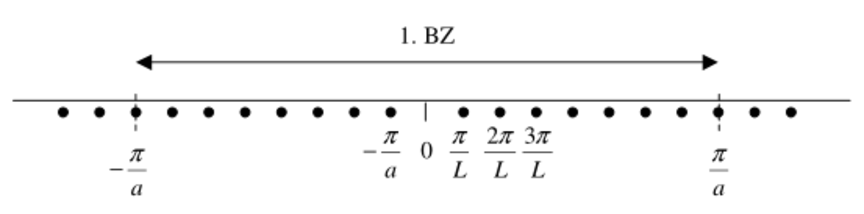
\includegraphics{ressources/Brillouin.pdf}
  \caption{Darstellung der ersten Brillouin-Zone für eine Kette mit 8 Einheitszellen, \cite{skript}.}
  \label{fig:Brill}
\end{figure}

In jeder dieser Zonen sind $2L/a$ k-Punkte mit
\begin{align}
  k=\frac{\pi}{L}
  \label{eq:k}
\end{align}
enthalten. Zu beachten ist, dass die Anzahl der Einheitszellen in der Brillouin-Zone der doppelten Anzahl der k-Punkte entspricht und bei $k=0$ keine Resonanzfrequenz für ein System endlicher Länge entsteht.

\subsubsection{Superstrukturen}
Als Superstrukturen werden periodische Störungen innerhalb eines periodischen Gitters bezeichnet. Diese periodische Störung wird durch einen Translationsvektor beschrieben, der einem ganzzahligen Vielfache des ursprünglichen Gittervektors entspricht. Dies kann beispielsweise eine Modifikation jeder zweiten Einheitszelle sein. Die Folge sind größere Gittervektoren und kleinere Brillouin-Zonen. Solche Formen von Störungen spielen z.B. im Bereich der Kondensierten Materie eine wichtige Rolle.

\subsubsection{Gitterfehler}
Durch Störungen, die die Periodizität des Gitters lokal zerstören, entstehen auch bei nur kleinen Störungen neue Zustände in den Bandlücken. Diese Methode wird dazu verwendet in Halbleitern Donator- oder Akzeptor-Level einzubringen.
% 2x2 Plot
% \begin{figure*}
%     \centering
%     \begin{subfigure}[b]{0.475\textwidth}
%         \centering
%         \includegraphics[width=\textwidth]{Abbildungen/Schaltung1.pdf}
%         \caption[]%
%         {{\small Schaltung 1.}}
%         \label{fig:Schaltung1}
%     \end{subfigure}
%     \hfill
%     \begin{subfigure}[b]{0.475\textwidth}
%         \centering
%         \includegraphics[width=\textwidth]{Abbildungen/Schaltung2.pdf}
%         \caption[]%
%         {{\small Schaltung 2.}}
%         \label{fig:Schaltung2}
%     \end{subfigure}
%     \vskip\baselineskip
%     \begin{subfigure}[b]{0.475\textwidth}
%         \centering
%         \includegraphics[width=\textwidth]{Abbildungen/Schaltung4.pdf}    % Zahlen vertauscht ... -.-
%         \caption[]%
%         {{\small Schaltung 3.}}
%         \label{fig:Schaltung3}
%     \end{subfigure}
%     \quad
%     \begin{subfigure}[b]{0.475\textwidth}
%         \centering
%         \includegraphics[width=\textwidth]{Abbildungen/Schaltung3.pdf}
%         \caption[]%
%         {{\small Schaltung 4.}}
%         \label{fig:Schaltung4}
%     \end{subfigure}
%     \caption[]
%     {Ersatzschaltbilder der verschiedenen Teilaufgaben.}
%     \label{fig:Schaltungen}
% \end{figure*}
